\chapter{Analiza wyników}
Program był tworzony, testowany oraz wykonywany na komputerze posiadającym 4 rdzeniowy procesor Intel Core i7-6700HQ oraz pamięć 8 GB (SO-DIMM DDR4, 2133MHz).

\section{Wygenerowane wykresy}
\label{wynik:wykres}
W celu analizy otrzymanych danych, program został uruchomiony pewną ilość razy, za każdym razem z innymi danymi wejściowymi. Otrzymane wykresy przedstawiają zmianę ilości elektronów znajdujących się w pułapkach w czasie trwania symulacji.

\begin{figure}[H]
\centering
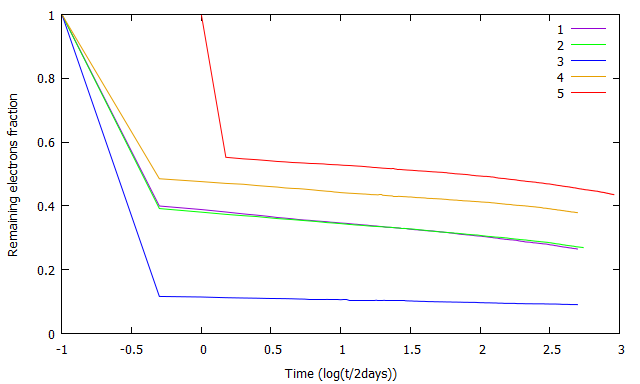
\includegraphics[width=17cm, height = 10cm]{wykres_all}
\caption{Porównanie otrzymanych wartości z różnymi parametrami wejściowymi}
\label{rys:1}
\end{figure}
\begin{itemize}
\item 1 - Ilość elektronów: $10^{4}$, ilość dziur elektronowych: $2*10^{4}$, zakres w którym losowane są położenia cząstek: [-1000,1000], symulowany czas: 1000 dni. Czas wykonania: 9 h.
\item 2 - Ilość elektronów: $2*10^{4}$, ilość dziur elektronowych: $3*10^{4}$, zakres w którym losowane są położenia cząstek: [-1100,1100], symulowany czas: 1100 dni. Czas wykonania: 24 h.
\item 3 - Ilość elektronów: $10^{4}$, ilość dziur elektronowych: $10^{4}$, zakres w którym losowane są położenia cząstek: [-400,400], symulowany czas: 1000 dni. Czas wykonania: 5 min.
\label{wykres:1}
\item 4 - Ilość elektronów: $10^{4}$, ilość dziur elektronowych: $10^{4}$, zakres w którym losowane są położenia cząstek: [-800,800], symulowany czas: 1000 dni. Czas wykonania: 3 h.
\label{wykres:2}
\item 5 - Ilość elektronów: $10^{4}$, ilość dziur elektronowych: $10^{4}$, zakres w którym losowane są położenia cząstek: [-900,900], symulowany czas: 5 lat. Czas wykonania: 13 h.
\end{itemize}


\begin{figure}[H]
\centering
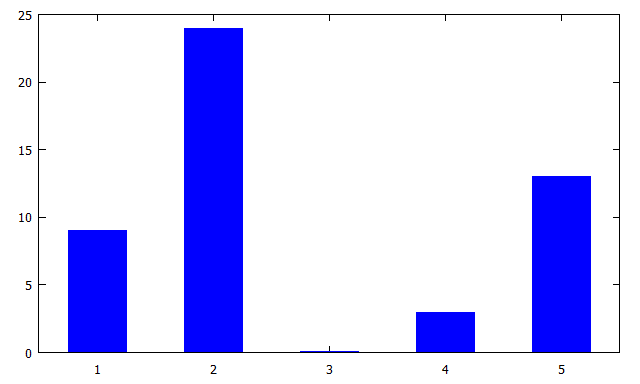
\includegraphics[width=17cm, height = 10cm]{czas}
\caption{Porównanie czasu wykonywania programu różnymi parametrami wejściowymi (w godzinach)}
\label{rys:1}
\end{figure}



\section{Analiza wykresów}
Analizując otrzymane wykresy można zauważyć znaczny spadek ilości elektronów w pułapkach na samym początku wykonywania programu. Jest to spowodowane faktem, że wszystkie współrzędne cząstek są losowane z podanego zakresu. Oznacza to, że na początku symulacji wiele pułapek elektronowych zawierających elektrony znajduje się bardzo blisko centrów rekombinacji. Powołując się na równania \ref{eq:1} oraz \ref{eq:2} obserwujemy, że odległość między pułapką a centrum rekombinacji znacząco wpływa na prawdopodobieństwo zajścia efektu tunelowego, co skutkuje zaobserwowanym początkowym spadkiem ilości wzbudzonych elektronów. Po wystąpieniu znaczącego spadku można zaobserwować, że ilość elektronów znajdujących się w pułapkach zaczyna maleć z dużo mniejszą częstotliwością. Wykres zaczyna wtedy przypominać funkcję liniową. 

Można przewidywać, że jeśli uruchomiono by symulację obrazującą dłuższy okres np. 50 lat, zanik elektronów w stanie wzbudzonym odbywałby się coraz wolniej. Wynika to z założenia, że elektron może przetunelować tylko jeden raz - oznacza to, że jeśli po pewnym czasie część elektronów przetuneluje do centrum rekombinacji, dla pozostałych elektronów prawdopodobieństwo zajścia tego efektu - które w głównej mierze zależy od odległości pomiędzy pułapką z elektronem, a pułapką z dziurą - będzie zbyt małe.

Ważnym parametrem symulacji jest zakres z którego losowane są wartości położenia dla cząstek. Porównując ze sobą wygenerowane dane na wykresie  \hyperref[wykres:1]{3} oraz \hyperref[wykres:2]{4} z rysunku \hyperref[rys:1]{4.1} gdzie ilość elektronów oraz symulowany czas są takie same, a zakres wartości położeń cząstki znacząco się różni, zaobserwowano, że im większa gęstość ładunków tym efekt tunelowania zachodzi szybciej, co jest zgodne z przewidywaniami wynikającymi ze wzoru \ref{eq:2}. Dzięki temu, oraz wykorzystanej implementacji wraz z założeniem że po zrekombinowaniu elektron nie może przetunelować po raz kolejny, czas wykonania programu zmniejszył się widocznie z 3h do ok. 5min. 
